% \documentclass[english, draft]{article}
\documentclass[english]{article}

\usepackage{geometry}
\usepackage{float}
\usepackage[utf8]{inputenc}
\usepackage[backend=biber,style= authoryear]{biblatex}
\usepackage[english]{babel}
\usepackage{csquotes}
\usepackage{graphicx}
\usepackage{subcaption}
\usepackage{booktabs}
\usepackage{xargs}
\usepackage[pdftex,dvipsnames,table]{xcolor}
\usepackage{bbold}

\graphicspath{{./resources/images}}
\addbibresource{../articles.bib}
\addbibresource{../manual.bib}

\geometry{a4paper, total={165mm,257mm}, left=15mm, top=20mm,}

\begin{document}
\pagenumbering{arabic}

\begin{abstract}

\end{abstract}

\section{Background}
European grapevine (Vitis vinifera L.) is one of the most economically and widespread worldwide crop. Around 33 of the  10.000 varieties,  cover 50% of the world's vineyard surface (OIV, 2017).
Grapevine faces numerous pathogens and one of the most damaging diseases is downy mildew, caused by the oomycete Plasmopara viticola. This pathogen is endemic to the North America and was introduced into Europe around the 1870s (Gessler et al., 2011., Fontaine et al., 2021). All the Vitis vinifiera varieties are susceptible to the pathogen and the current strategy to control the disease  relies on the massive applications of fungicides and which are potentially harmful for the humans and the environment. Long -lasting breeding programs have been conducted to introgress resistance from wild Vitis species into elite resistant varieties (Merdinoglu et al., 2018; Töpfer & Trapp, 2022). According to Possamai & Wiedemann-Merdinoglu, (2022), more than 30 resistance genetic loci or Rpv (Resistance to Plasmopara viticola), have been already identified in grapevine and the majority of them confer a visual partial resistance defined by various levels of sporulation and  necrosis. The analysis of macroscopic phenotypes of the disease have been implemented by using several variables such as severity, incidence, spores count. Therefore, the use of the semi-quantitative OIV452-1 scale was frequently used assessing both sporulation and necrosis.

\section{Material and Method}

% Annotation a décrire dans le texte et parler des divergences et accords garder trace des désaccords et en parler lors de la discussion -> ML approaches can stabilise?
% Enlever tous les désaccords avant le modèle? : Combien de données restent peux-t'on entrainer uniquement avec ça
% Enlever seulement une partie des données fausse le but de l'expérience
% Quelle question on pause quel dataset pour y répondre
% Est-ce que les erreurs sont dans les images difficiles ?
% Matrice de confusion avec ou sans désacord
% Critique de l'OIV ? 7 & 9 neccessaires


% Tables & figures
% Légendes
% Fontes
% Nom de colonnes

\begin{figure}[H]
    \begin{center}
        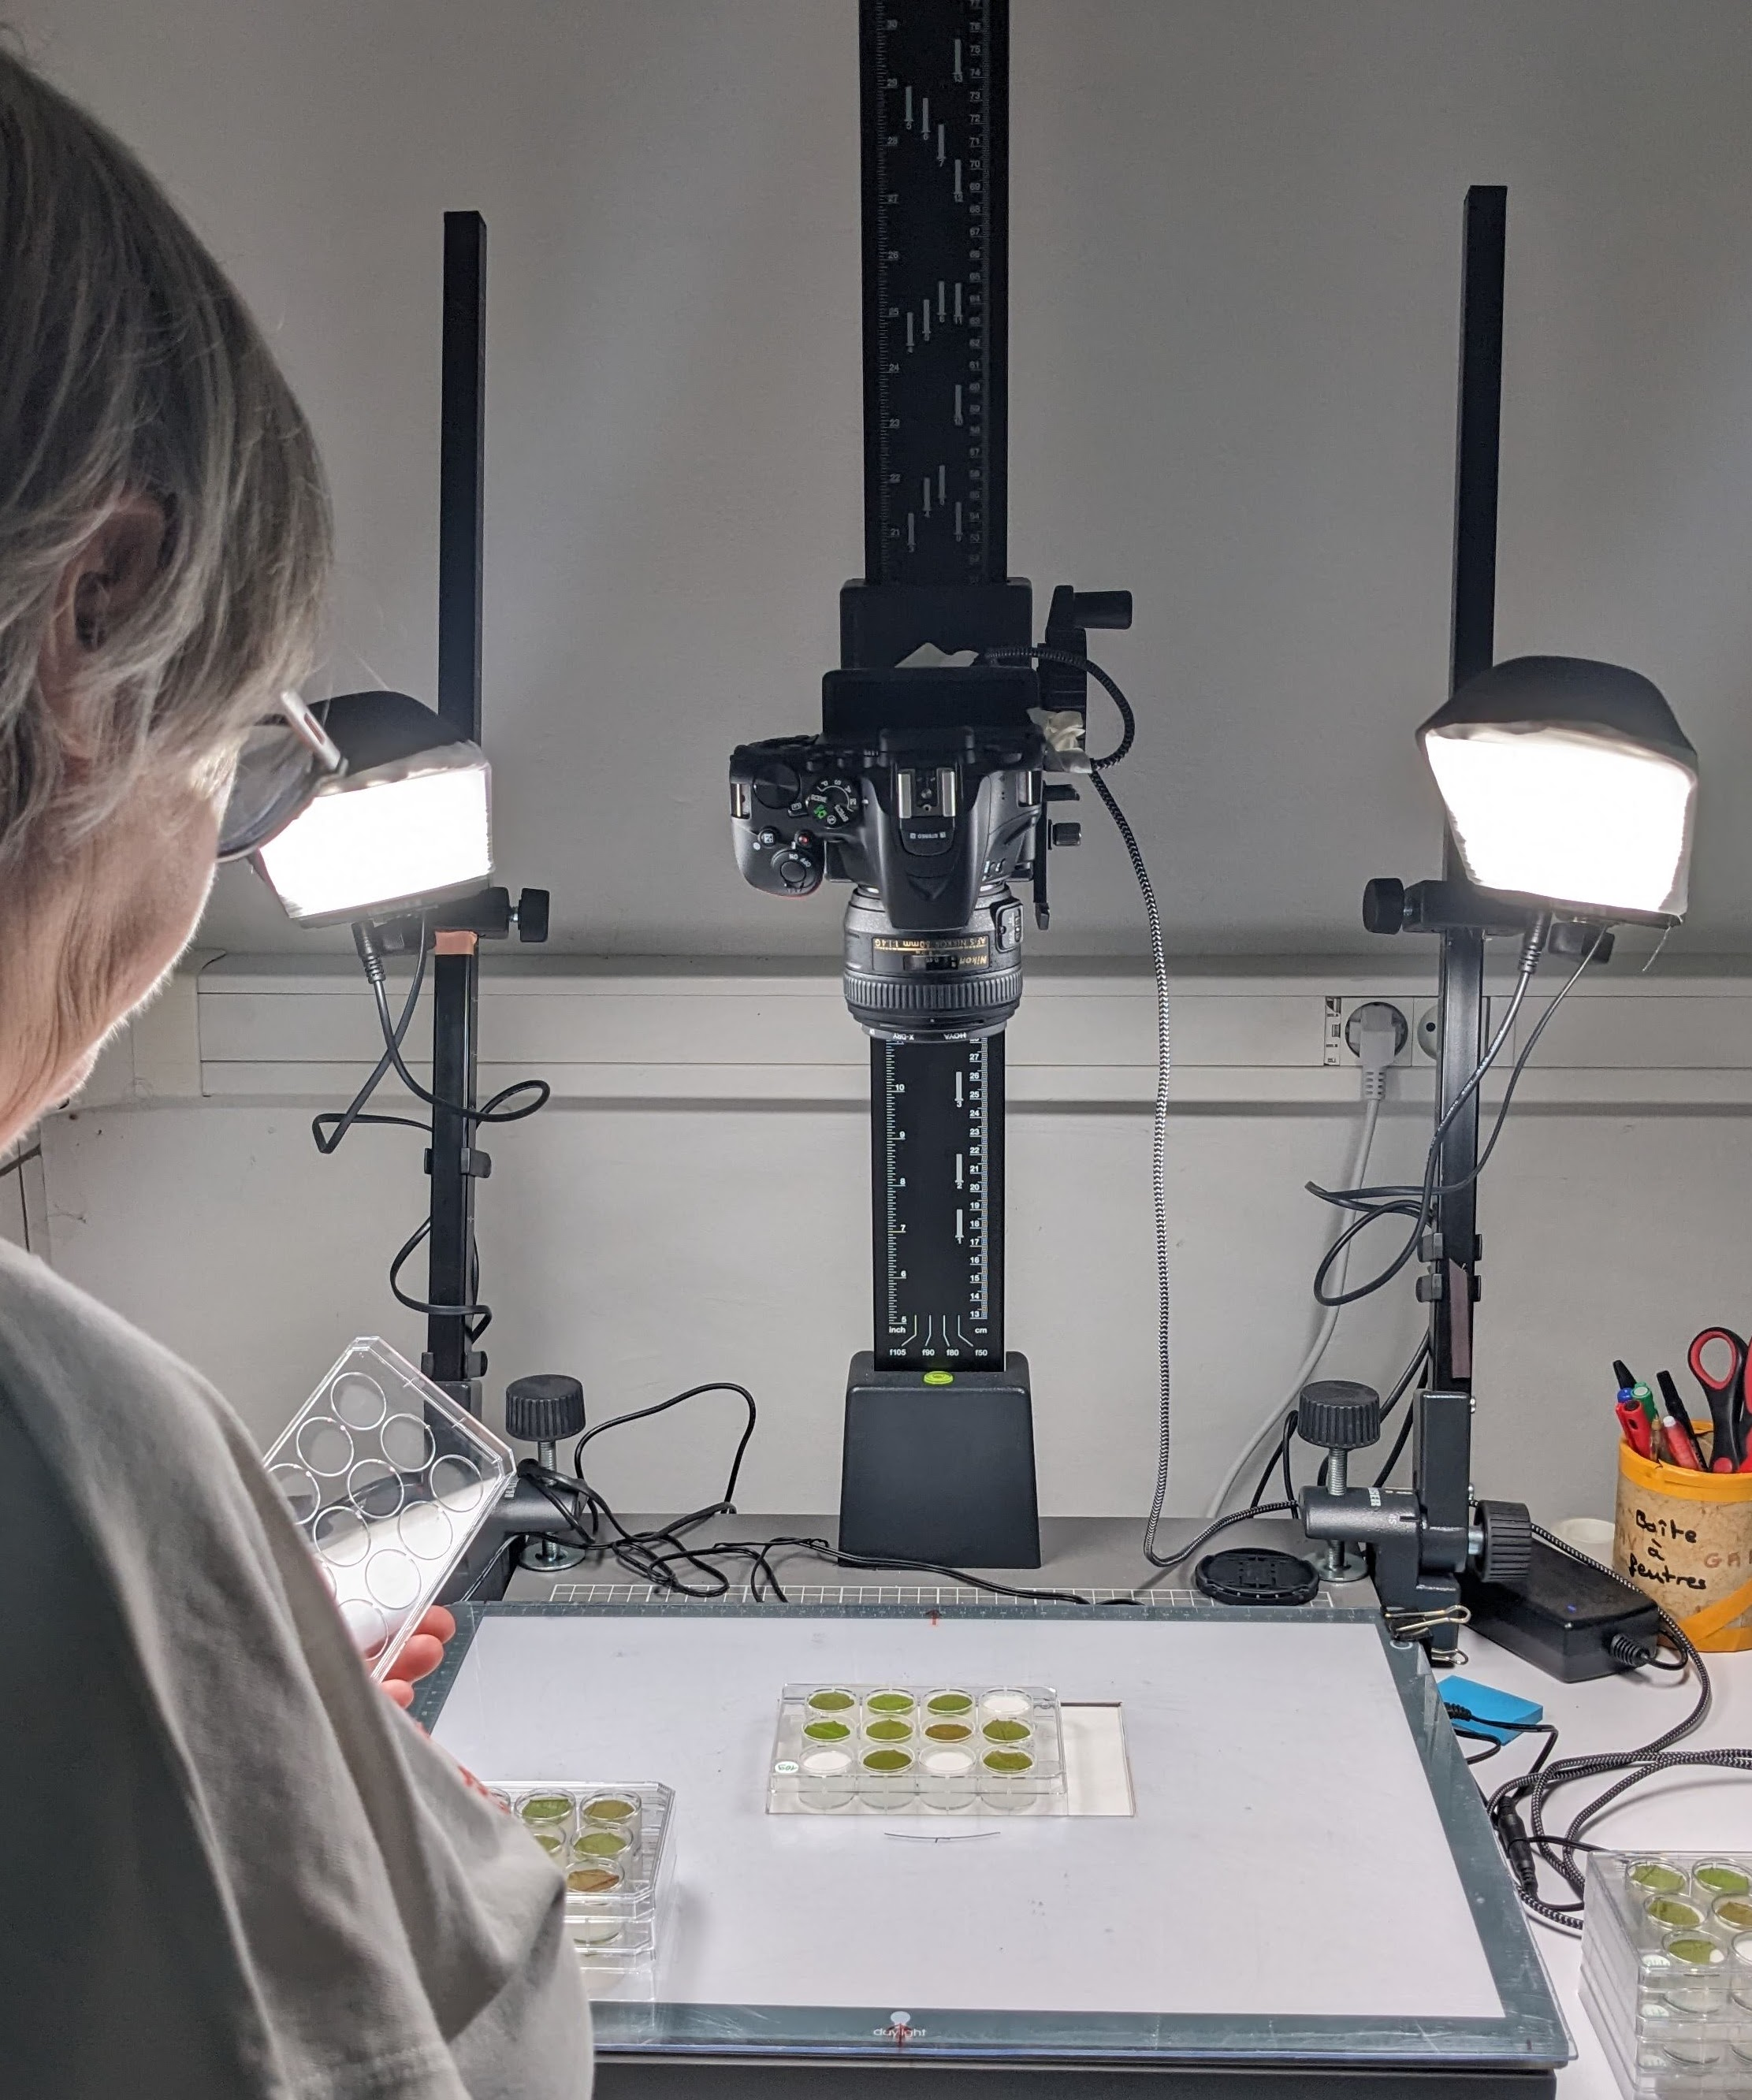
\includegraphics[width=0.5\linewidth]{2023_a_oiv_imaging_system.jpg}
        \caption{VEGOIA platform's manual imaging system}\label{fig:vegoia}
    \end{center}
\end{figure}

\begin{figure}[H]
    \centering
    \begin{subfigure}[b]{0.2\linewidth}
        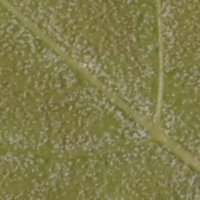
\includegraphics[width=\linewidth]{p_viticola/resources/images/2023_a_oiv_sporulation.png}
        \caption{Sporulation}\label{fig:sporulation}
    \end{subfigure}
    \begin{subfigure}[b]{0.2\linewidth}
        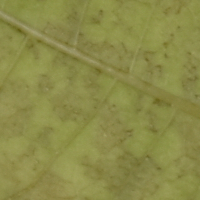
\includegraphics[width=\linewidth]{p_viticola/resources/images/2023_a_oiv_stains.png}
        \caption{Flecks}\label{fig:flecks}
    \end{subfigure}
    \begin{subfigure}[b]{0.2\linewidth}
        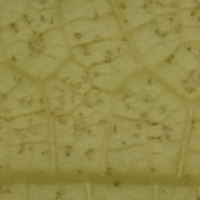
\includegraphics[width=\linewidth]{p_viticola/resources/images/2023_oiv_a_dots.png}
        \caption{Dots}\label{fig:dots}
    \end{subfigure}
    \begin{subfigure}[b]{0.2\linewidth}
        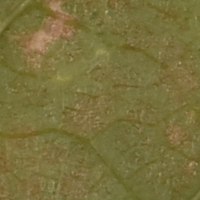
\includegraphics[width=\linewidth]{p_viticola/resources/images/2023_a_oiv_senescence.png}
        \caption{Senscence}\label{fig:senescence}
    \end{subfigure}
    \caption{Examples of \textit{Vitis} leaf discs infected with \textit{Plasmopara viticola} showing the four different phenotypes selected.}
\end{figure}

\begin{table}[H]
\centering
\caption{Distribution of image quality and annotations for phenotype detecttion}
\label{tab:databincount}
\begin{tabular}{lrrrr}
\toprule
 issue &  sporulation &  necrosis\_dots &  necrosis\_stains &  necrosis\_senescence \\
\midrule
  blur &           11 &             10 &                2 &                    7 \\
colour &           23 &              0 &                0 &                   13 \\
  good &          983 &            579 &              261 &                  374 \\
 water &          102 &            118 &               25 &                   49 \\
 total &         1119 &            712 &              289 &                  444 \\
\bottomrule
\end{tabular}
\end{table}

\begin{figure}[H]
    \centering
    \begin{subfigure}[b]{0.3\linewidth}
        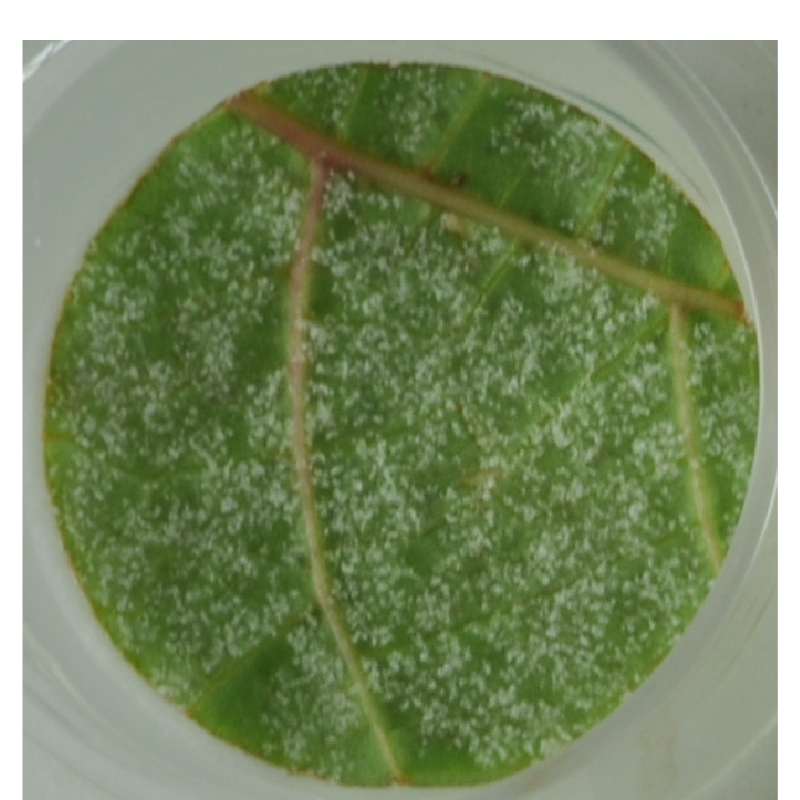
\includegraphics[width=\linewidth]{oiv1.png}
        \caption{OIV 1}\label{fig:oiv1}
    \end{subfigure}
    \begin{subfigure}[b]{0.3\linewidth}
        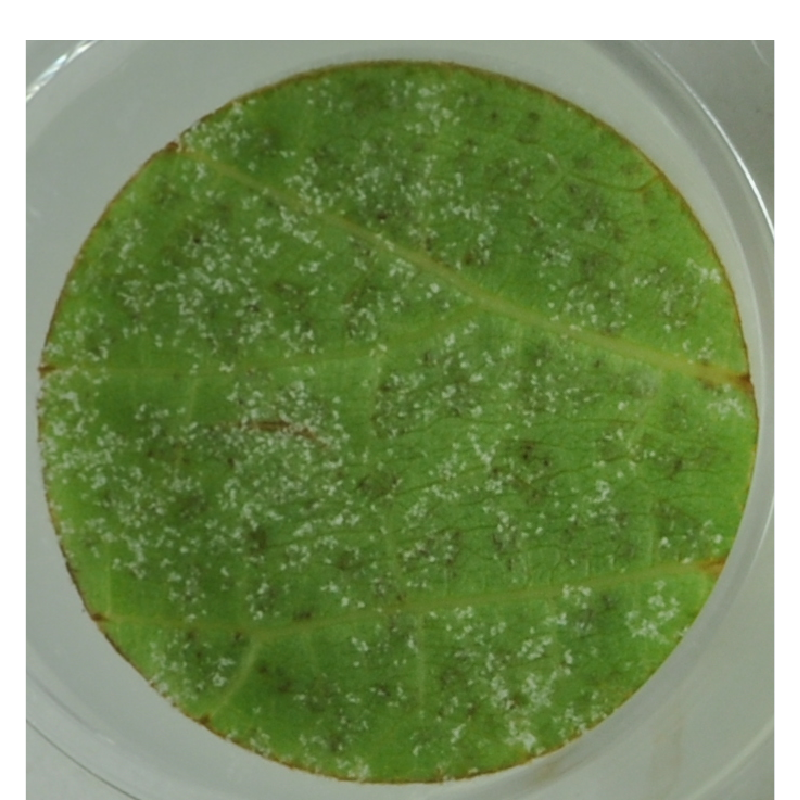
\includegraphics[width=\linewidth]{oiv3.png}
        \caption{OIV 3}\label{fig:oiv3}
    \end{subfigure}
    \begin{subfigure}[b]{0.3\linewidth}
        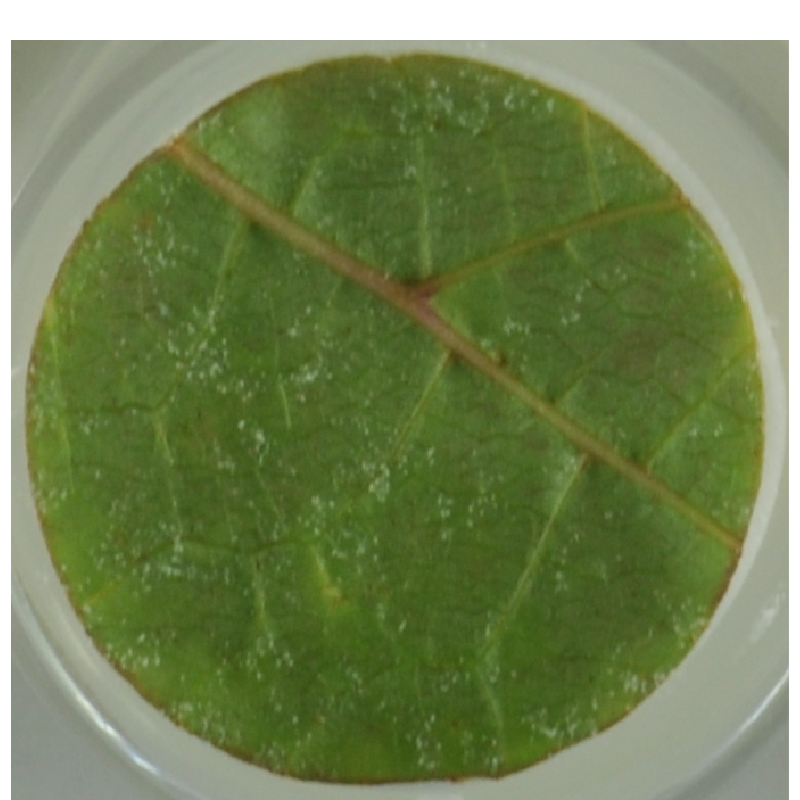
\includegraphics[width=\linewidth]{oiv5.png}
        \caption{OIV 5}\label{fig:oiv5}
    \end{subfigure}
    \begin{subfigure}[b]{0.3\linewidth}
        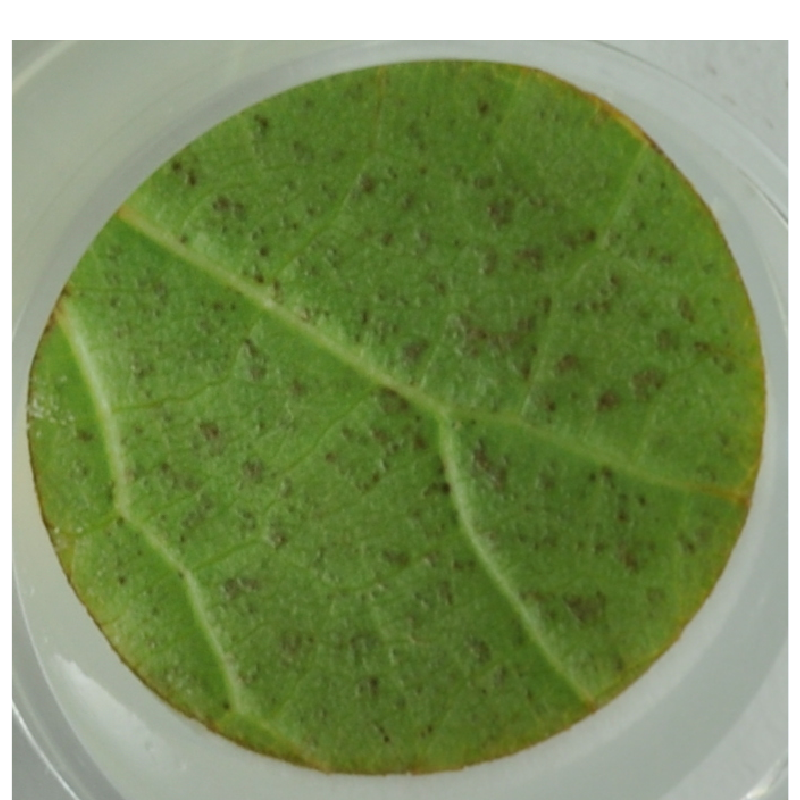
\includegraphics[width=\linewidth]{oiv7.png}
        \caption{OIV 7}\label{fig:oiv7}
    \end{subfigure}
    \begin{subfigure}[b]{0.3\linewidth}
        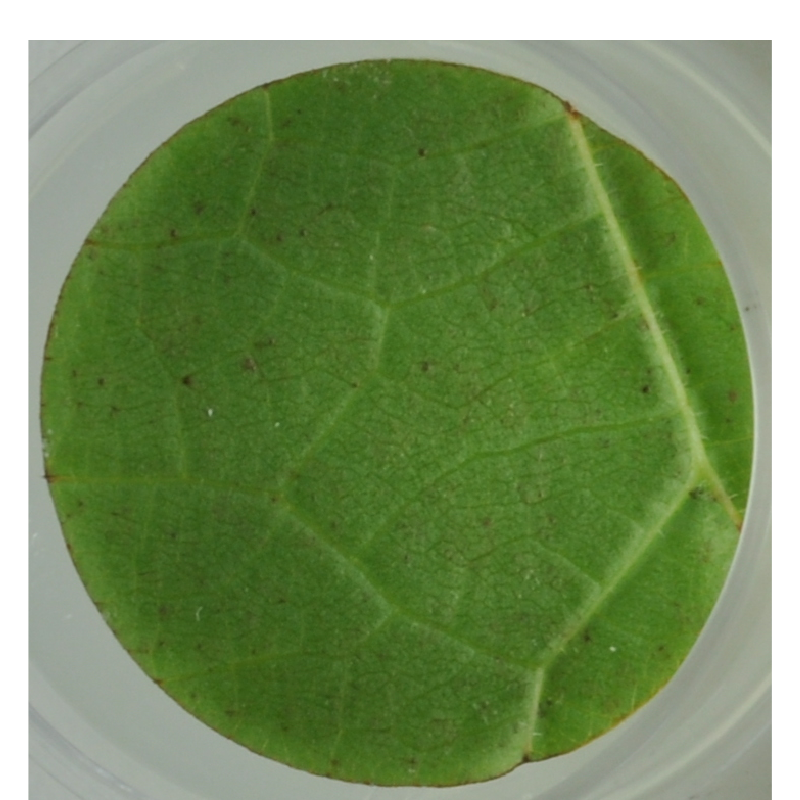
\includegraphics[width=\linewidth]{oiv9.png}
        \caption{OIV 9}\label{fig:oiv9}
    \end{subfigure}
    \caption{Examples of \textit{Vitis} leaf discs infected with \textit{Plasmopara viticola} annotated with OIV 452-1 values. Levels increase with resistance to pathogen. Upper row, susceptible leaf discs with levels 1 to 5. Lower row, resistant leaf disc~\ref{fig:oiv7} and fully resistant leaf disc~\ref{fig:oiv9}}\label{fig:phenotypes}
\end{figure}

\begin{table}[H]
\centering
\caption{Distribution of image quality and OIV values}
\label{tab:dataoivcount}
\begin{tabular}{rrrrrrrr}
\toprule
 oiv &  blur &  color &  crop &  dark &  good &  water &  total \\
\midrule
   1 &     0 &      0 &     3 &    10 &   626 &    116 &    755 \\
   3 &     2 &      2 &     0 &     7 &   479 &    144 &    634 \\
   5 &     3 &      1 &     0 &     5 &   412 &    146 &    567 \\
   7 &     1 &      0 &     3 &     6 &   549 &    141 &    700 \\
   9 &     0 &      0 &     4 &    12 &   513 &    331 &    860 \\
\bottomrule
\end{tabular}
\end{table}


\begin{figure}[H]
    \begin{center}
        \includegraphics[width=0.9\linewidth]{p_viticola/resources/images/leaf_disc_extraction_2.png}
        \caption{Leaf disc extraction workflow}\label{fig:preprocessing}
    \end{center}
\end{figure}


\begin{equation}
    L = -\sum_{c=1}^My_{o,c}\log(p_{o,c})\label{fml:crossentropy}
\end{equation}

\begin{figure}[H]
    \centering
    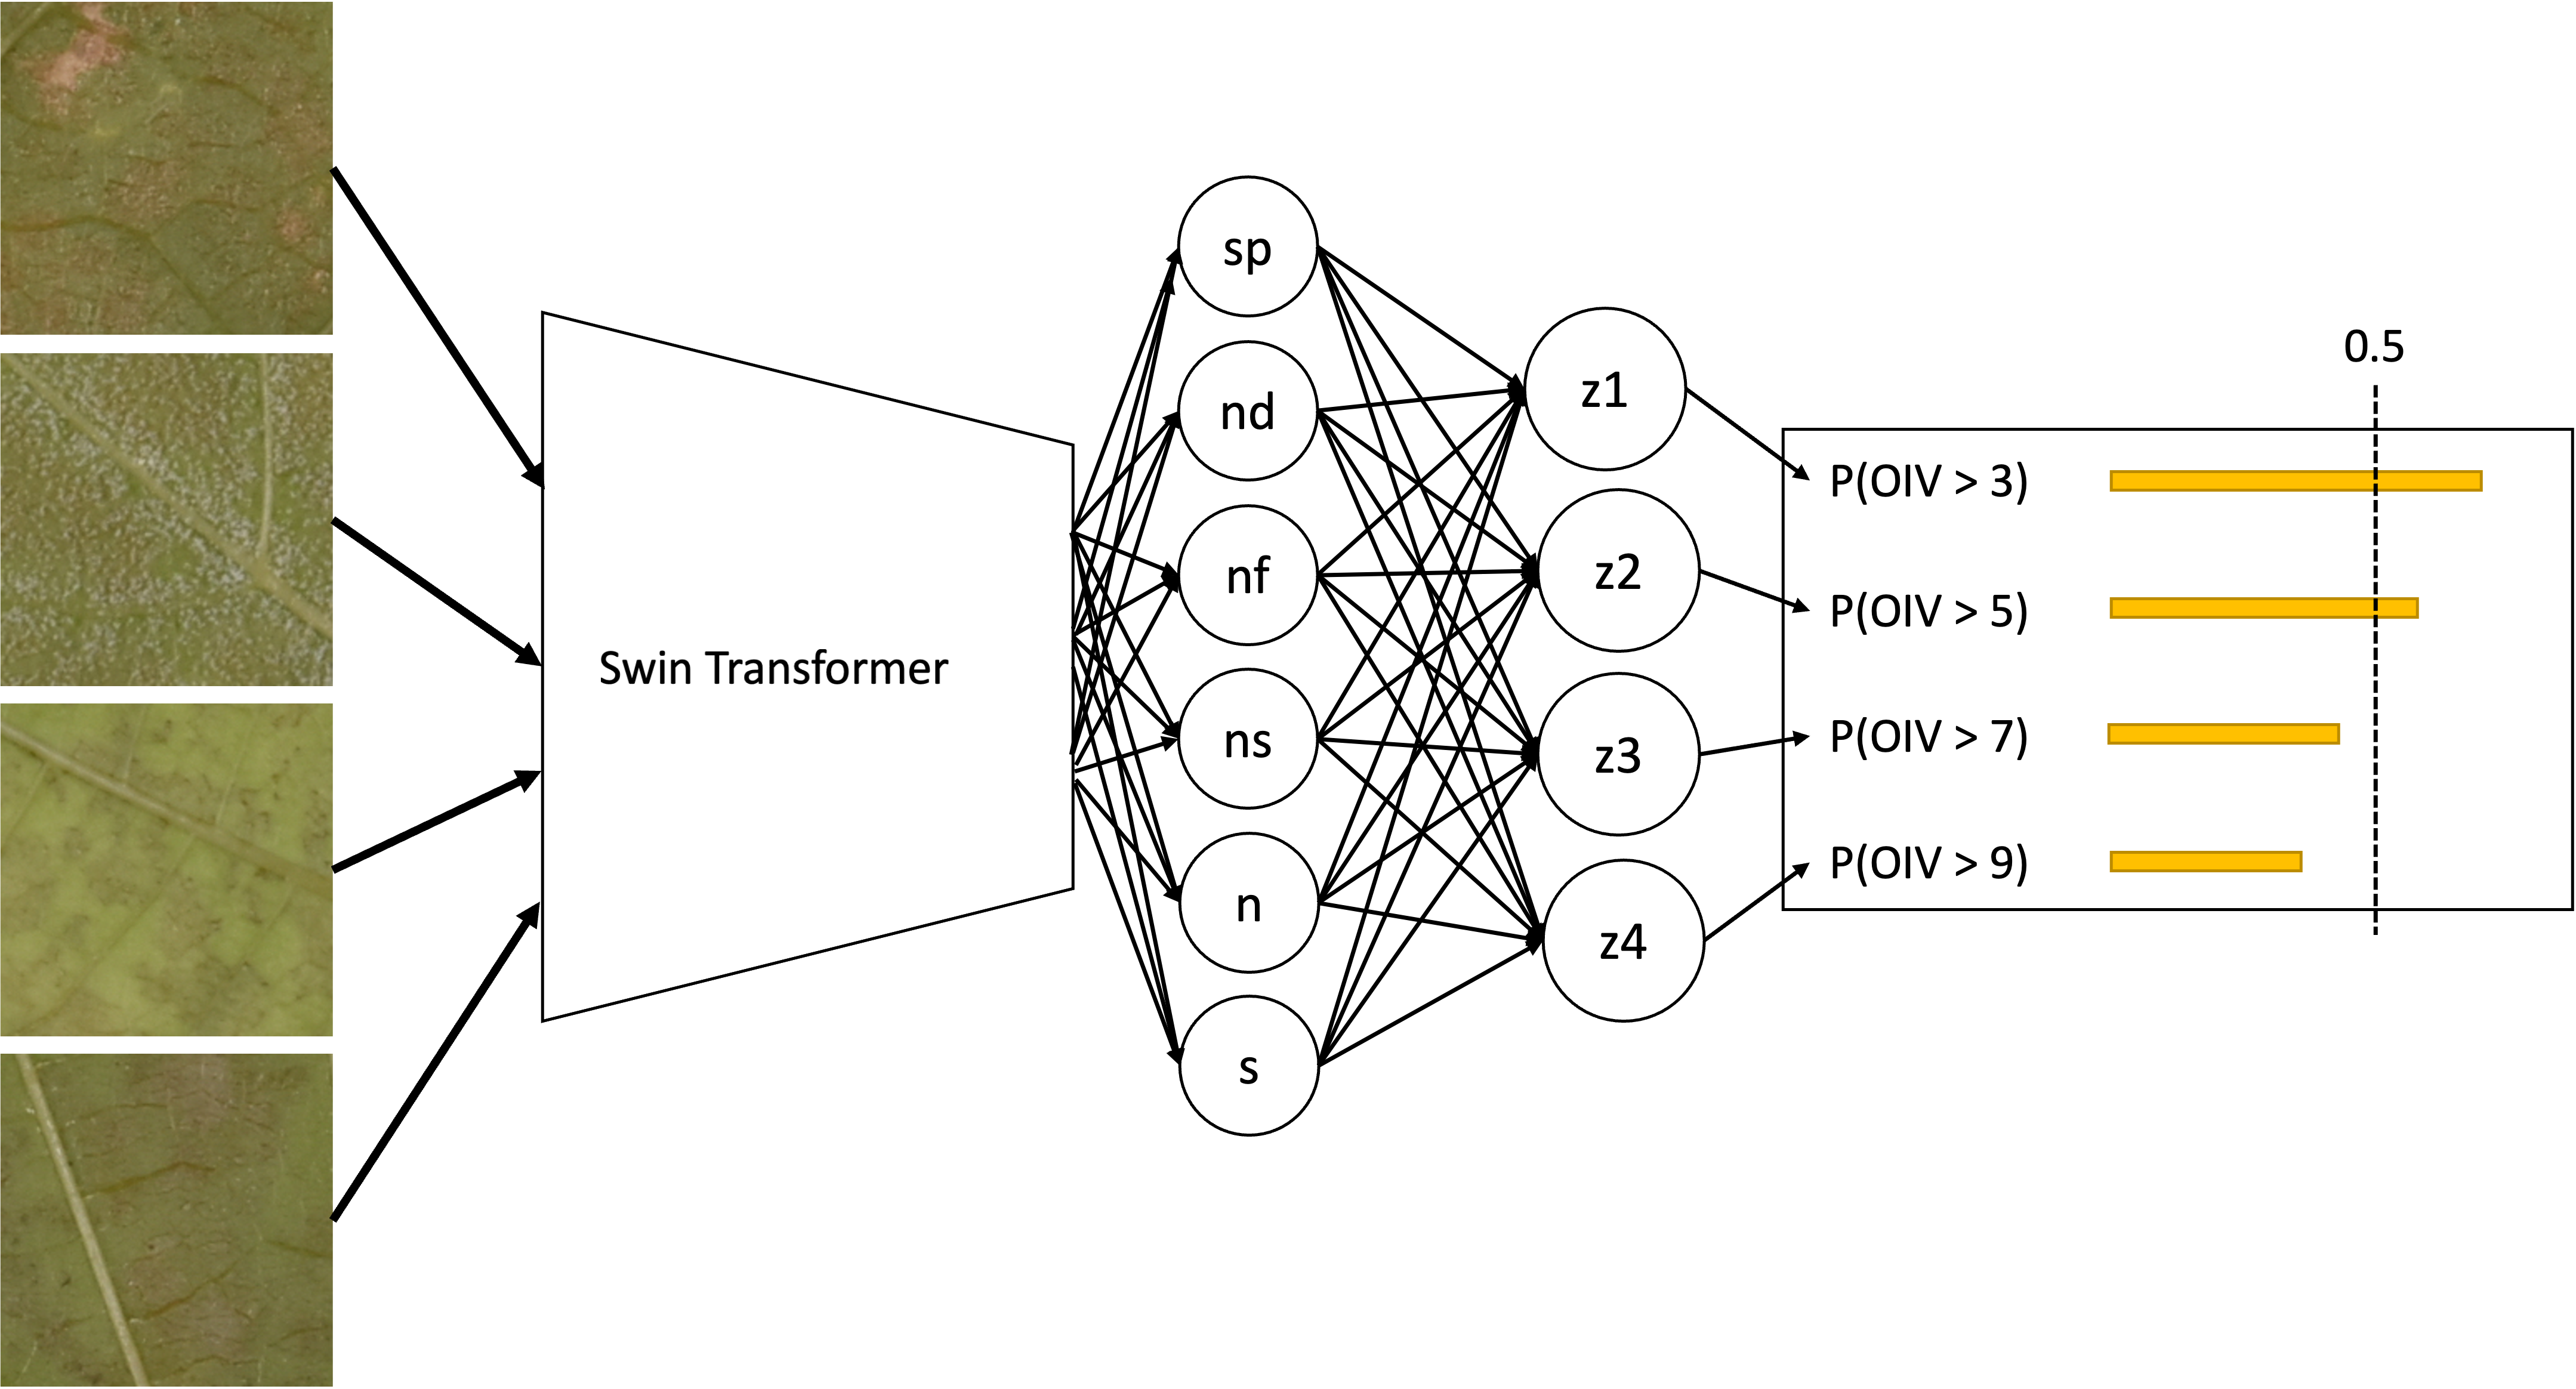
\includegraphics[width=0.9\linewidth]{p_viticola/resources/images/2023_a_oiv_bin_corn.png}
    \caption{Rank-consistent ordinal regression (CORN) architecture with output example predicting OIV 7}
    \label{fig:corn}
\end{figure}

\begin{equation}
    f(x^{[i]}) = \hat{P}(y^{[i]} > r_{k}|y^{[i]} > r_{k-1})\label{fml:binclass}
\end{equation}

\begin{equation}
    \hat{P}(y^{[i]} > r_{k}) = \prod_{j=1}^{k}f_{j}(x^{[i]})\label{fml:unconditionalprob}
\end{equation}

\begin{equation}
    OIV = (\sum_{j=1}^{K-1}\mathbb{1}(\hat{P}(y^{[i]} > r_{j}) > 0.5))*2 + 1\label{fml:rankprob}
\end{equation}

\section{Results and Discussion}

\subsection{Leaf Disc Detection}

\begin{table}[H]
\centering
\caption{Leaf disc detection models evaluation}
\label{tab:leafdiscdetectionresult}
\begin{tabular}{lrrrrr}
\toprule
{} & \multicolumn{5}{l}{val\_loss} \\
{} &    count &    min &    mean & median &         std \\
scheduler &          &        &         &        &             \\
\midrule
None      &       20 &  0.015 &  0.0176 &  0.017 &  0.00223371 \\
steplr    &       15 &  0.012 &  0.0154 &  0.015 &  0.00213140 \\
\bottomrule
\end{tabular}
\end{table}

\subsection{Binary Predictions}
\begin{figure}[H]
    \centering
    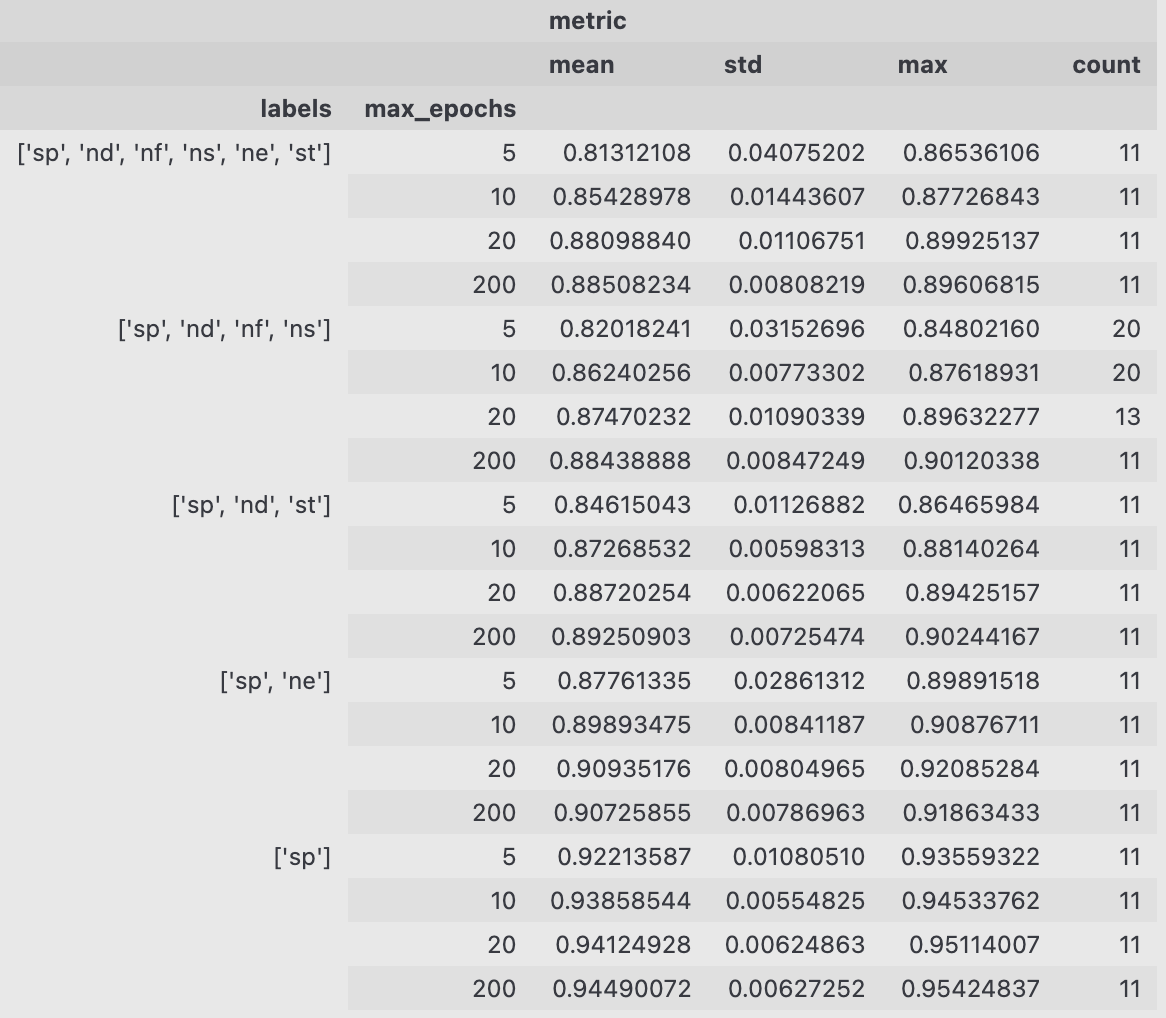
\includegraphics[width=0.9\linewidth]{p_viticola//resources//images/binary_models_result.png}
    \caption{Backbones training results}
    \label{fig:binbackbones}
\end{figure}


\subsection{OIV prediction}

\begin{figure}[H]
    \centering
    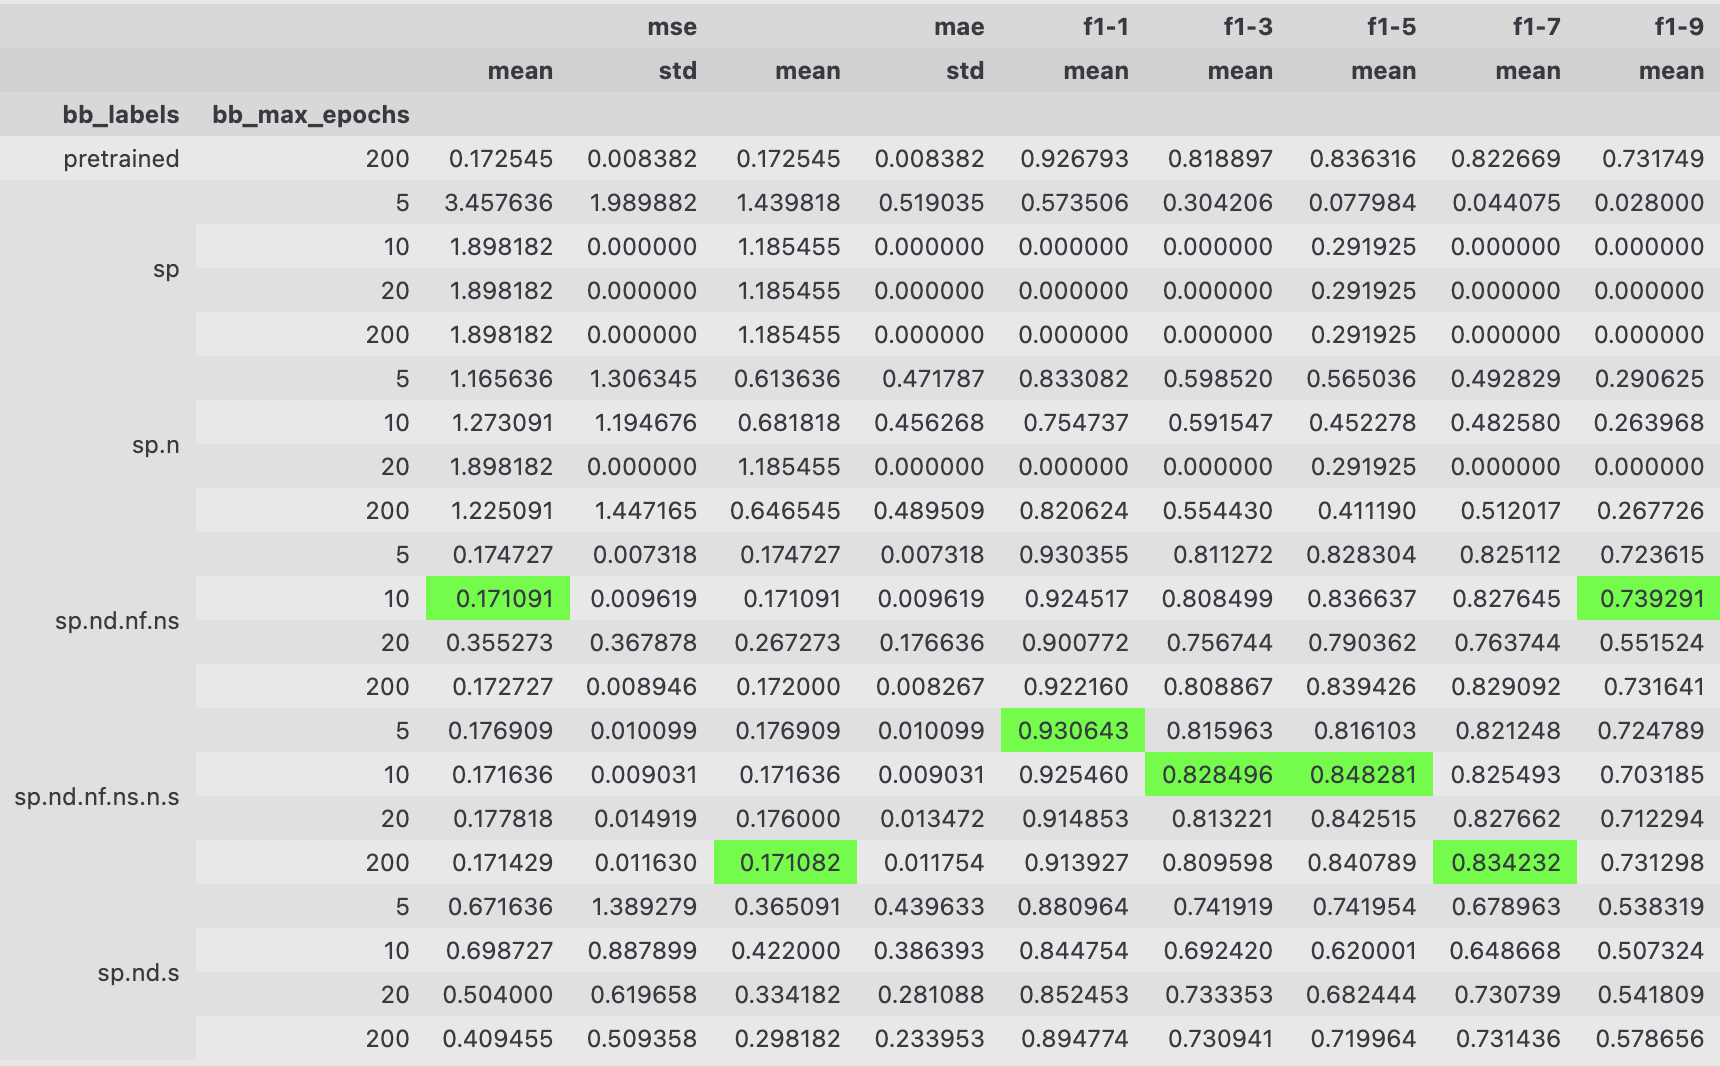
\includegraphics[width=0.9\linewidth]{p_viticola//resources//images/oivresult.png}
    \caption{OIV predictors evaluation}
    \label{fig:oivresultstable}
\end{figure}


\begin{figure}[H]
    \centering
    \begin{subfigure}[b]{0.45\linewidth}
        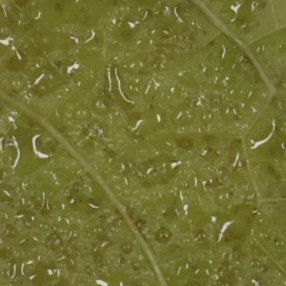
\includegraphics[width=\linewidth]{water.png}
        \caption{Water droplets may be mistaken with sporulation}\label{fig:error97water}
    \end{subfigure}
    \begin{subfigure}[b]{0.45\linewidth}
        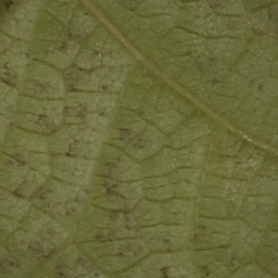
\includegraphics[width=\linewidth]{error_97.png}
        \caption{White stains appear in image}\label{fig:error97b}
    \end{subfigure}
    \caption{Images with OIV value 9 predicted as 7}\label{fig:errors97}
\end{figure}

\begin{figure}[H]
    \centering
    \begin{subfigure}[b]{0.45\linewidth}
        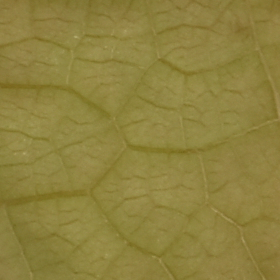
\includegraphics[width=\linewidth]{error_79_2.png}
        \caption{}\label{fig:error79a}
    \end{subfigure}
    \begin{subfigure}[b]{0.45\linewidth}
        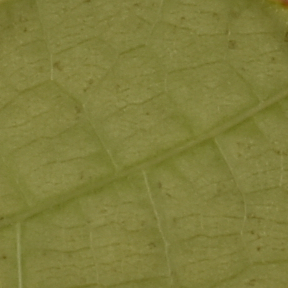
\includegraphics[width=\linewidth]{error_79_1.png}
        \caption{}\label{fig:error79b}
    \end{subfigure}
    \caption{Images with OIV value 7 predicted as 9 when sporulation is hardly perceptible}\label{fig:errors79}
\end{figure}

\subsection{New Experiment}

\begin{figure}[H]
    \centering
    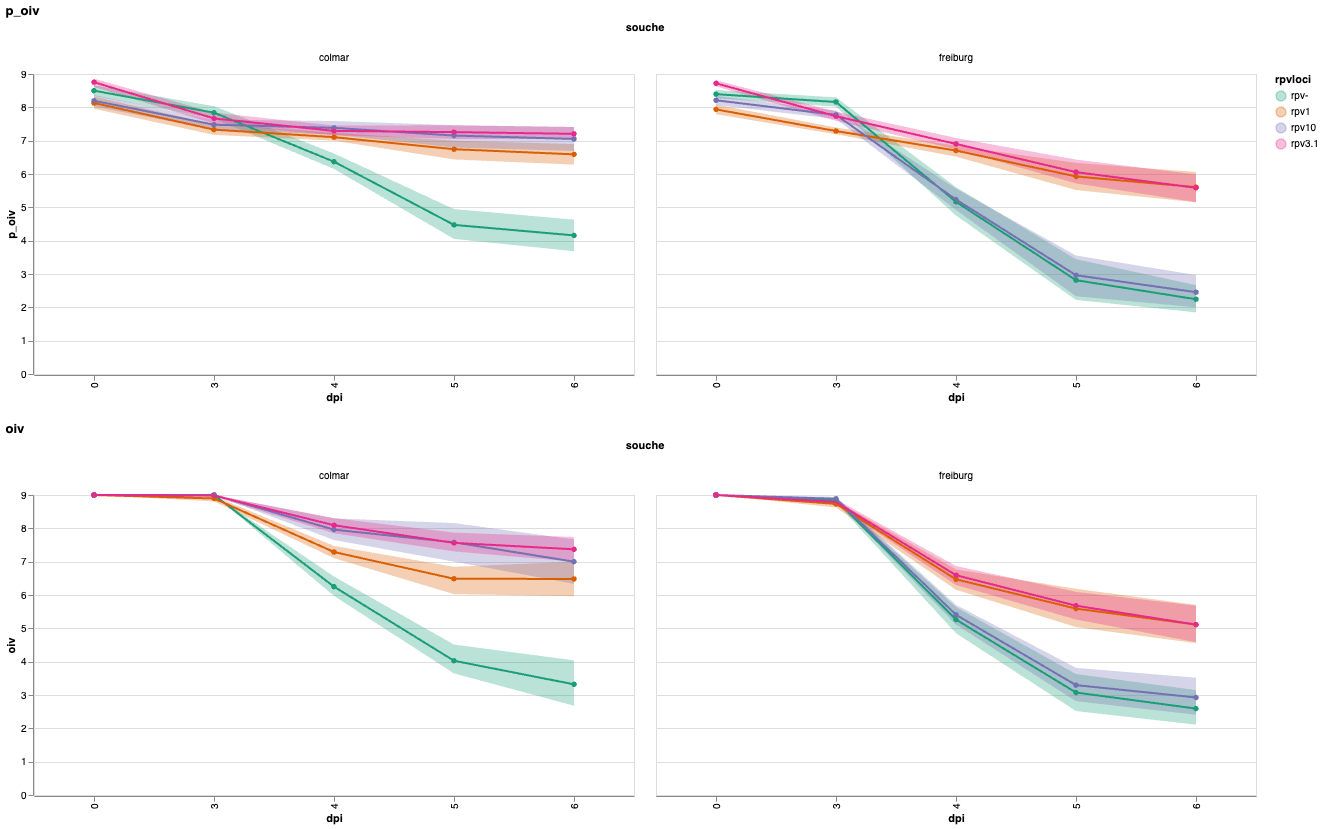
\includegraphics[width=0.9\linewidth]{p_viticola/resources/images/dm23.png}
    \caption{Model inference on never seen experimental data}
    \label{fig:2023DM89}
\end{figure}

\section{Conclusions and perspectives}




\end{document}